\part{Technical description}
\chapter{Hardware}
\section{Introduction to CSE1}
The CS Enterprise I was initially bought in 2009, as a fully configured model boat named "Aziz" built by Model Slipway. Due to requirements for master and PhD experiments, the model was refitted by \cite{Skaatun2011}. The work performed on CS Enterprise I include, but is not limited to, dynamic positioning systems, maneuvering systems and path following, and navigation with virtual reality.

The vessel is a 1:50 scale model of a tug boat, and is fitted with two Voith Schneider propellers(VSP) astern and one bow thruster(BT). The main dimensions of the vessel are:
\begin{table}[h!]
	\caption{Main dimensions of CSE1}
	\centering
	\begin{tabular}{cc}
		\hline
		LOA & 1.105[m]\\
		B & 0.248 [m]\\
		$\Delta$ & 14.11 [kg]\\\hline
	\end{tabular}
\end{table}

\subsection{Literature}
The development of CSE1 is a product of much research from several theses, which contain complementary information on the theory applied to the system. 
\subsubsection{Journals and conferences}
\begin{itemize}
	\item LOS guidance for towing an iceberg along a straight-line path \citep{OrstenNorgrenSkjetne2014}
\end{itemize}
\subsubsection{Specialization projects and master theses}
\begin{itemize}
	\item Development of a DP system for CS Enterprise I with Voith Schneider thrusters. \citep{Skaatun2011}
	\item Development of a modularized control architecture for CS Enterprise I for path-following based on LOS and maneuvering theory \citep{Tran2013}
	\item Automatic Reliability-based Control of Iceberg Towing in Open Waters \citep{Orsten2014}
	\item Line-Of-Sight-based maneuvering control design, implementation, and experimental testing for the model ship C/S Enterprise I.\citep{Tran2014}
	\item Remote Control and Automatic Path-following for C/S Enterprise I and ROV Neptunus \citep{Sandved2015}
	\item Marine Telepresence System \citep{Valle2015}
	\item Nonlinear Adaptive Motion Control and Model-Error Analysis for Ships-Simulations and MCLab experiments \citep{bjorne2016nonlinear}
	\item Low-Cost Observer and Path-Following Adaptive Autopilot for Ships \citep{mykland2017}
\end{itemize}
\subsubsection{Other}
\begin{itemize}
	\item YouTube video \citep{Skaatun2014}
\end{itemize}

\section{Actuators}
Figure \ref{fig:position_of_actuators} illustrate the position of the actuators, and their distance from CO is given in Table \ref{tab:thruster_distance}. The BT and VSP motor speeds are controlled by an Electronic Speed Control(ESC). The ESC receive their setpoints as pulse-width modulated (PWM) signals from the cRIO digital output module. The VSP blade pitches are controlled by servos. The servos also receive their setpoint as PWM signals.

\begin{minipage}{\textwidth}
	\begin{minipage}[b]{0.49\textwidth}
		\centering
		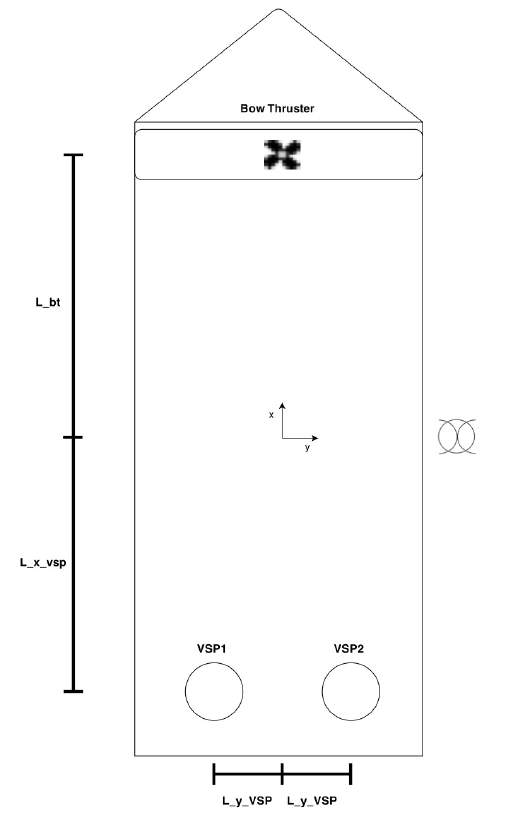
\includegraphics[width=\linewidth]{fig/actuators_overview.png}
		\captionof{figure}{Position of actuators. Adapted from \cite{Valle2015}}
		\label{fig:position_of_actuators}
	\end{minipage}
	\hfill
	\begin{minipage}[b]{0.49\textwidth}
		\centering
		\begin{tabular}{ccc}
		\hline
		\textbf{Parameter} & \textbf{Symbol} & \textbf{Value}[m]\\\hline
		x length to VSP & $L_{x,VSP}$ & -0.4574\\
		x length to BT & $L_{BT}$ & 0.3875\\
		y length to VSP & $L_{y,VSP}$ & 0.055\\\hline
		\end{tabular}
	\captionof{table}{Position of actuators}
	\label{tab:thruster_distance}
	\end{minipage}
\vspace{0.5cm}
\end{minipage}

\section{Power system}
CSE1 is powered with one 12V 12Ah battery on-board. Some of the components require different voltage, and thus some voltage converters are mounted. However, the setup works as it is, and by connecting the battery to the wires, the whole system is powered. A schematic of the power grid is illustrated in Figure \ref{fig: CSE1 power}, and Figure \ref{fig:battery_connected} show a photo of the battery mounted and connected. 
\begin{figure*}[htb!]
\centering
\begin{subfigure}{.45\linewidth}
	\centering
	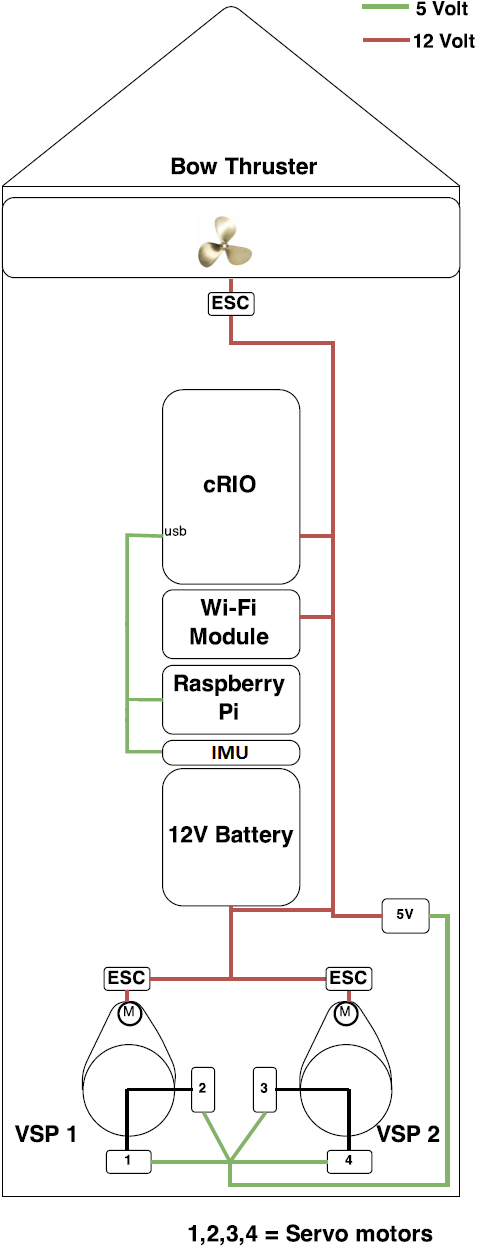
\includegraphics[height=0.4\paperheight]{fig/CSE1_power}
	\caption{CSE1 power system}
	\label{fig: CSE1 power}
\end{subfigure}
\begin{subfigure}{0.45\linewidth}
	\centering
	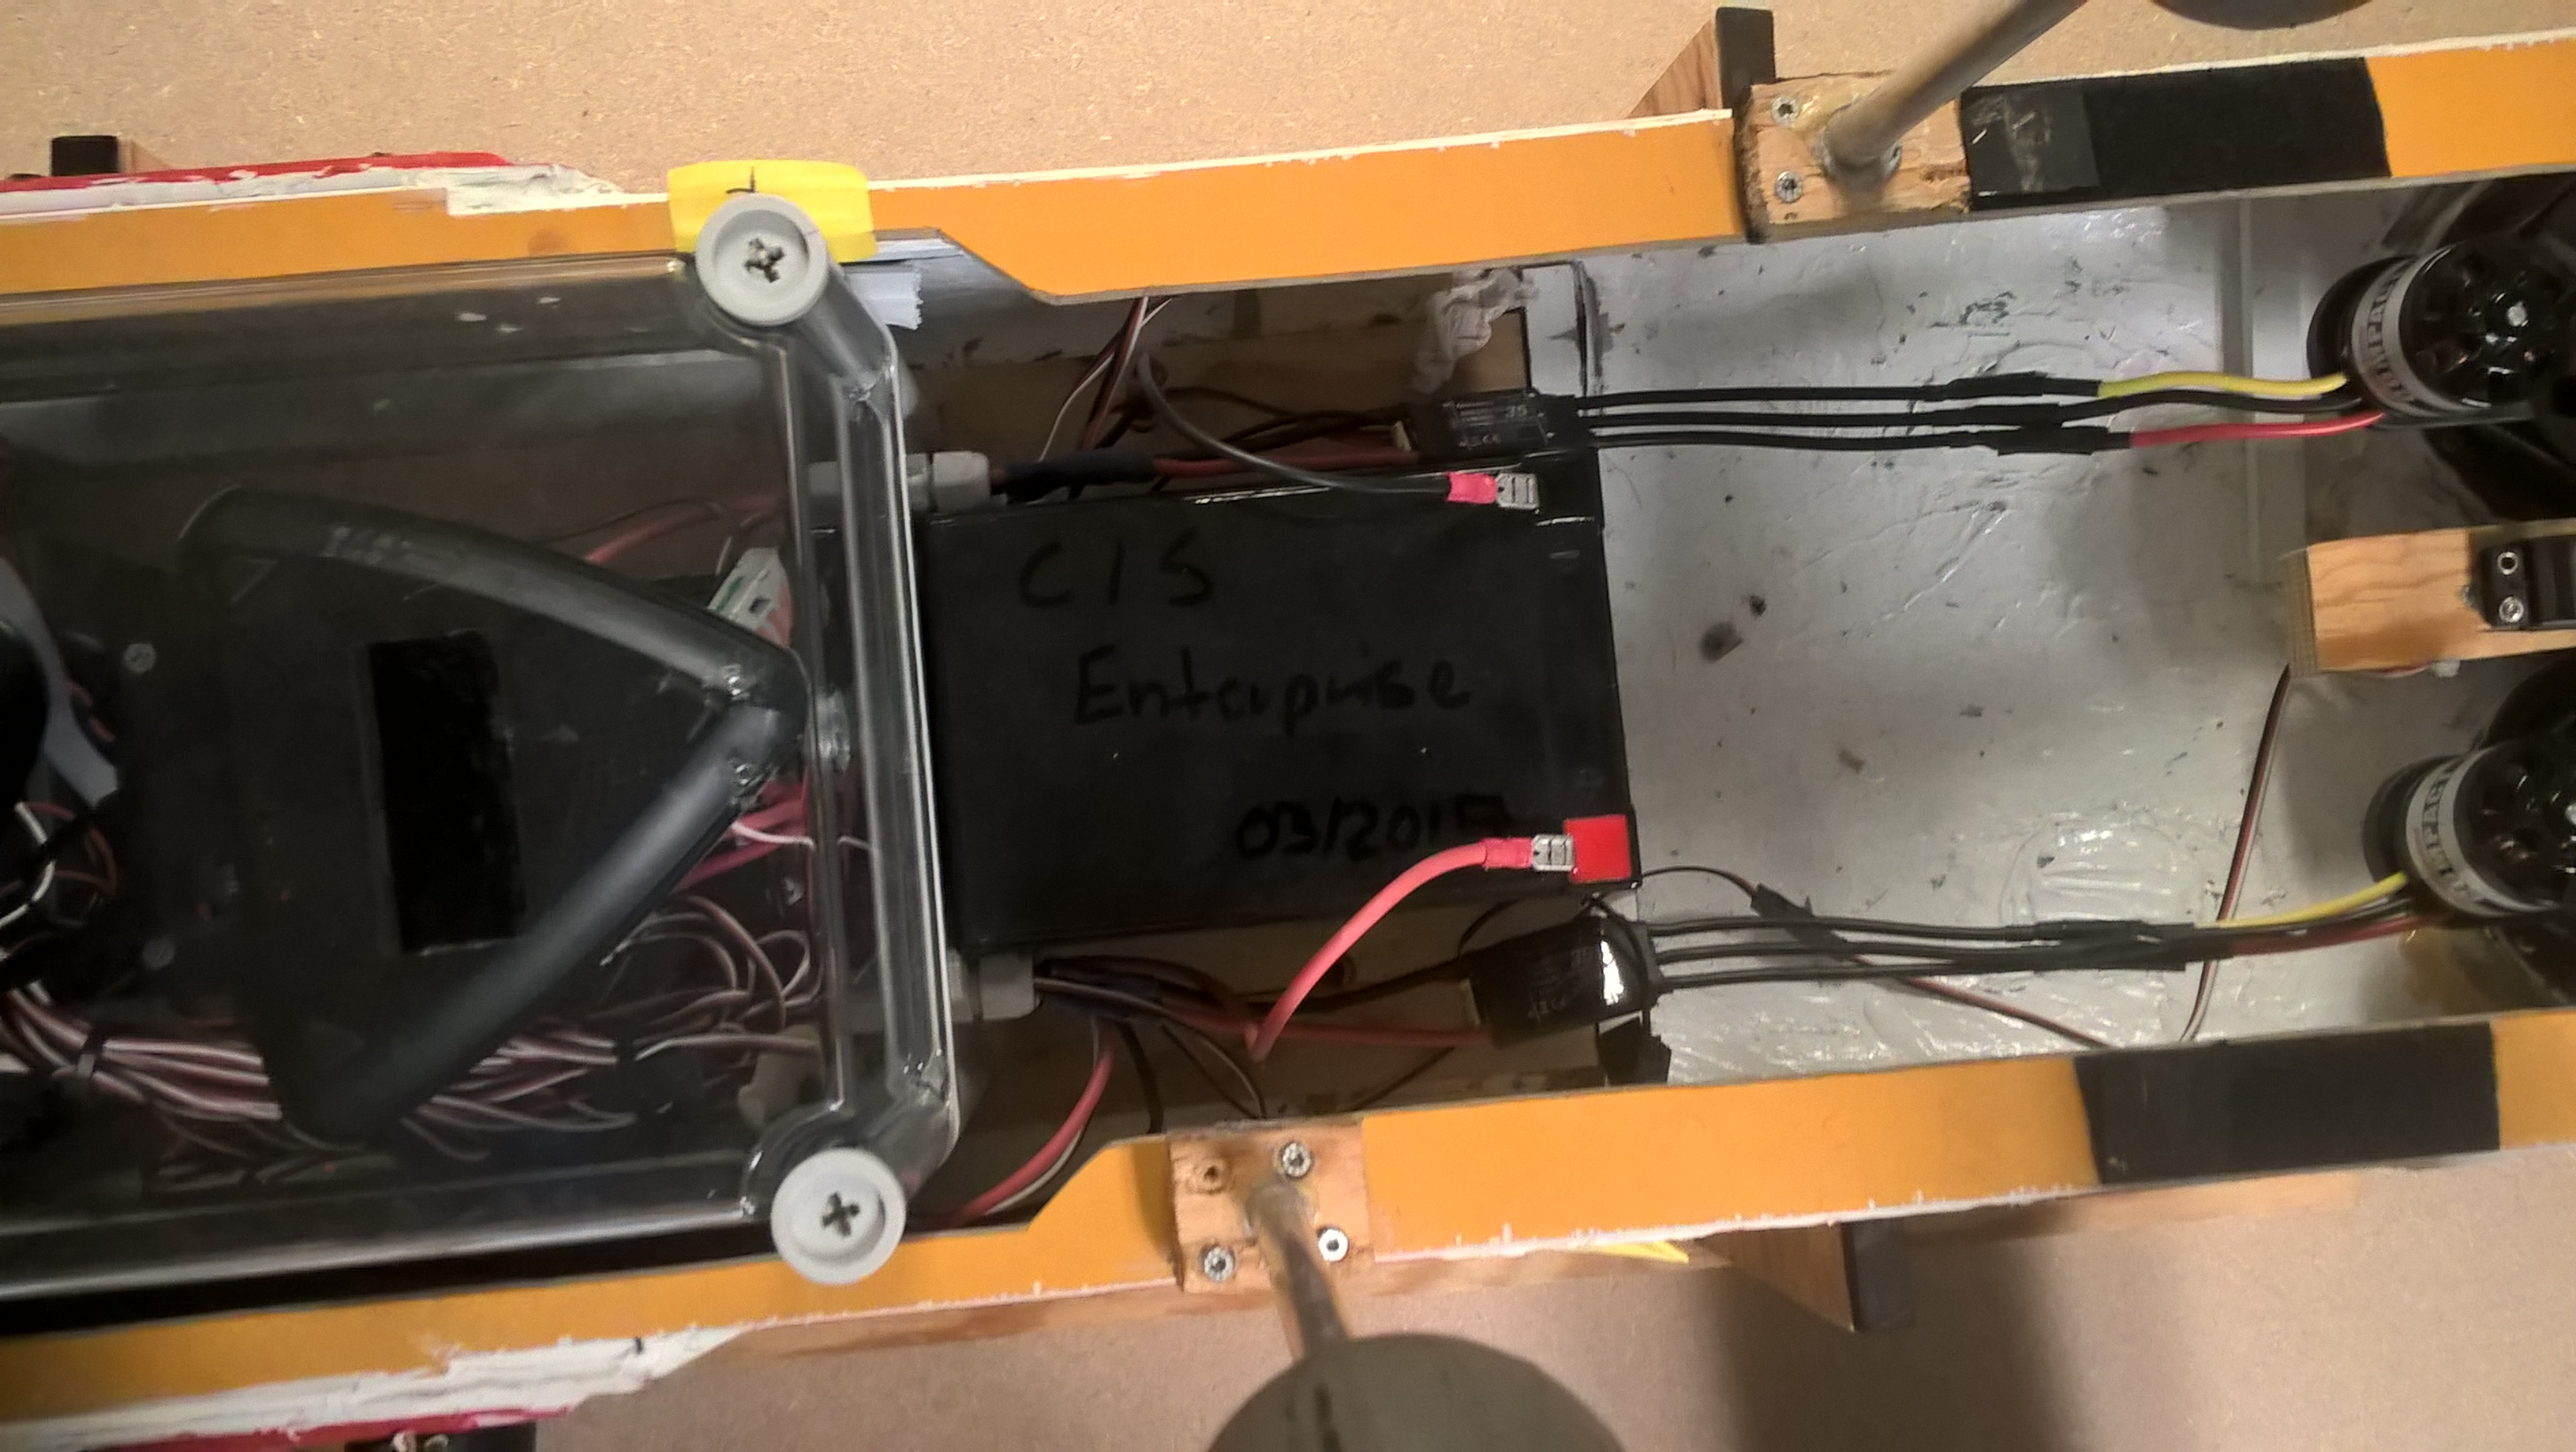
\includegraphics[width=\linewidth]{fig/battery_mounted.jpg}
	\caption{Battery mounted and connected}
	\label{fig:battery_connected}
\end{subfigure}
\caption{Battery system}
\end{figure*}

\section{IMU}
CSE1 is equipped with one Inertial Measurement Unit (IMU) from Analog Devices. The sensor mounted on-board is the ADIS16364 and includes a triaxis gyroscope and triaxis accelerometer. The sensor has built-in compensation for bias, alignment and sensitivity, and thus provides accurate measurements over a temperature range of -10 to +70 degrees Celsius. The sampling rate is set to 100 Hz. The most relevant data is presented in Table \ref{tab:IMU_specifications}, and for supplementary information the reader is referred to the data sheet \cite{adis16364}. The coordinate frame of the sensor is illustrated in Figure \ref{fig:IMU_reference_frame}, with positive directions illustrated by arrows. As seen, the standard coordinate frame for linear accelerations uses left-hand orientation, while the angular rates uses right-hand orientation. It is advised to change the coordinate frame of accelerations to right-hand, which is achieved by multiplying the accelerations with -1. Further, the sensor is mounted with a different orientation than the body frame, as can be seen in Figure \ref{fig:IMU_mounted}. Using the \textit{zyx}-convention, the sensor frame has an orientation relative body frame: $(\phi, \theta, \psi) = (\pi, 0, 0)$. Hence, by using the rotation matrix with these values, the measured accelerations and angular rates can be rotated to the body-frame. 
\begin{table}[htb!]\caption{IMU specifications}\label{tab:IMU_specifications}
	\centering
	\begin{tabular}{c|c|c|c|}
		\cline{2-4}
		& \textbf{Parameter} & \textbf{Typical value} & \textbf{Unit}\\ \cline{1-4}
		\multicolumn{1}{|c|}{\multirow{5}{*}{\textbf{Gyroscopes}}} & Dynamic range & $\pm 350$ & \degree/sec\\ 
		\multicolumn{1}{|c|}{} & Sensitivity & 0.0125 & \degree/sec/LSB\\ 
		\multicolumn{1}{|c|}{} & Bias stability, $\sigma$ & 0.007 & \degree/sec\\ 
		\multicolumn{1}{|c|}{} & Angular random walk & 2.0 & \degree/$\sqrt{hr}$\\ 
		\multicolumn{1}{|c|}{} & Output noise & 0.8 & \degree/sec rms\\ \cline{1-4}
		
		\multicolumn{1}{|c|}{\multirow{5}{*}{\textbf{Accelerometers}}} & Dynamic range & $\pm 5.25$ & g\\ 
		\multicolumn{1}{|c|}{} & Sensitivity & 1.00 & mg/LSB\\ 
		\multicolumn{1}{|c|}{} & Bias stability, $\sigma$ & 0.1 & mg\\ 
		\multicolumn{1}{|c|}{} & Velocity random walk & 0.12 & m/sec/$\sqrt{hr}$\\ 
		\multicolumn{1}{|c|}{} & Output noise & 5 & mg rms\\ \cline{1-4}
		
		\multicolumn{1}{|c|}{\multirow{1}{*}{\textbf{Power supply}}} & Operating voltage& $5.0 \pm 0.25$ & V\\ \cline{1-4}
	\end{tabular}
\end{table}
\begin{figure}[htb!]
	\centering
	\begin{subfigure}{0.45\linewidth}
		\centering
		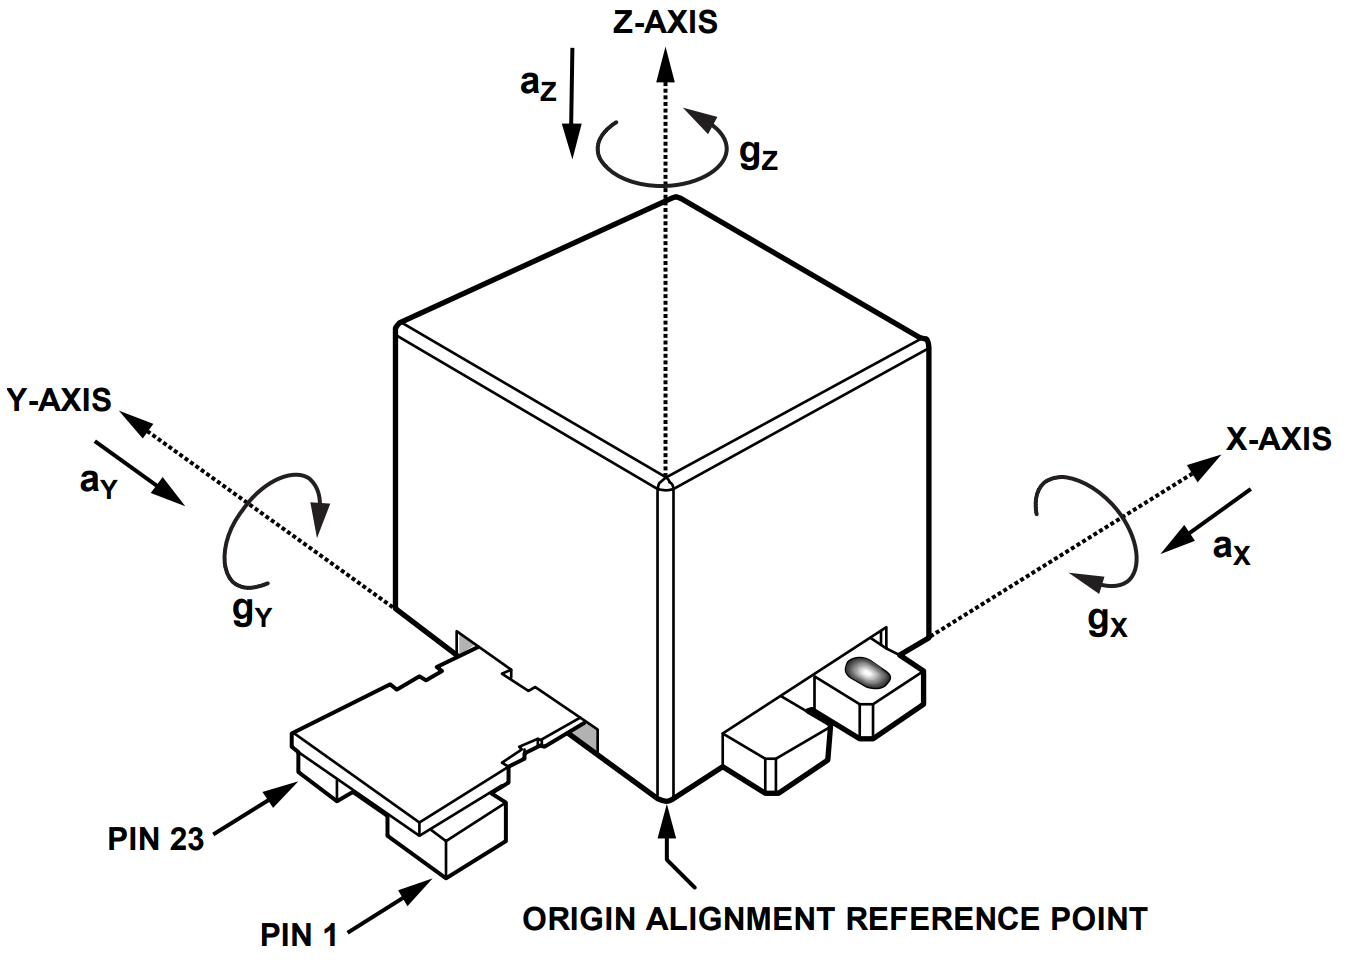
\includegraphics[width=1\linewidth]{fig/IMU_reference_frame.png}
		\caption{IMU reference frame from manufacturer}
		\label{fig:IMU_reference_frame}
	\end{subfigure}
	\begin{subfigure}{0.45\linewidth}
		\centering
		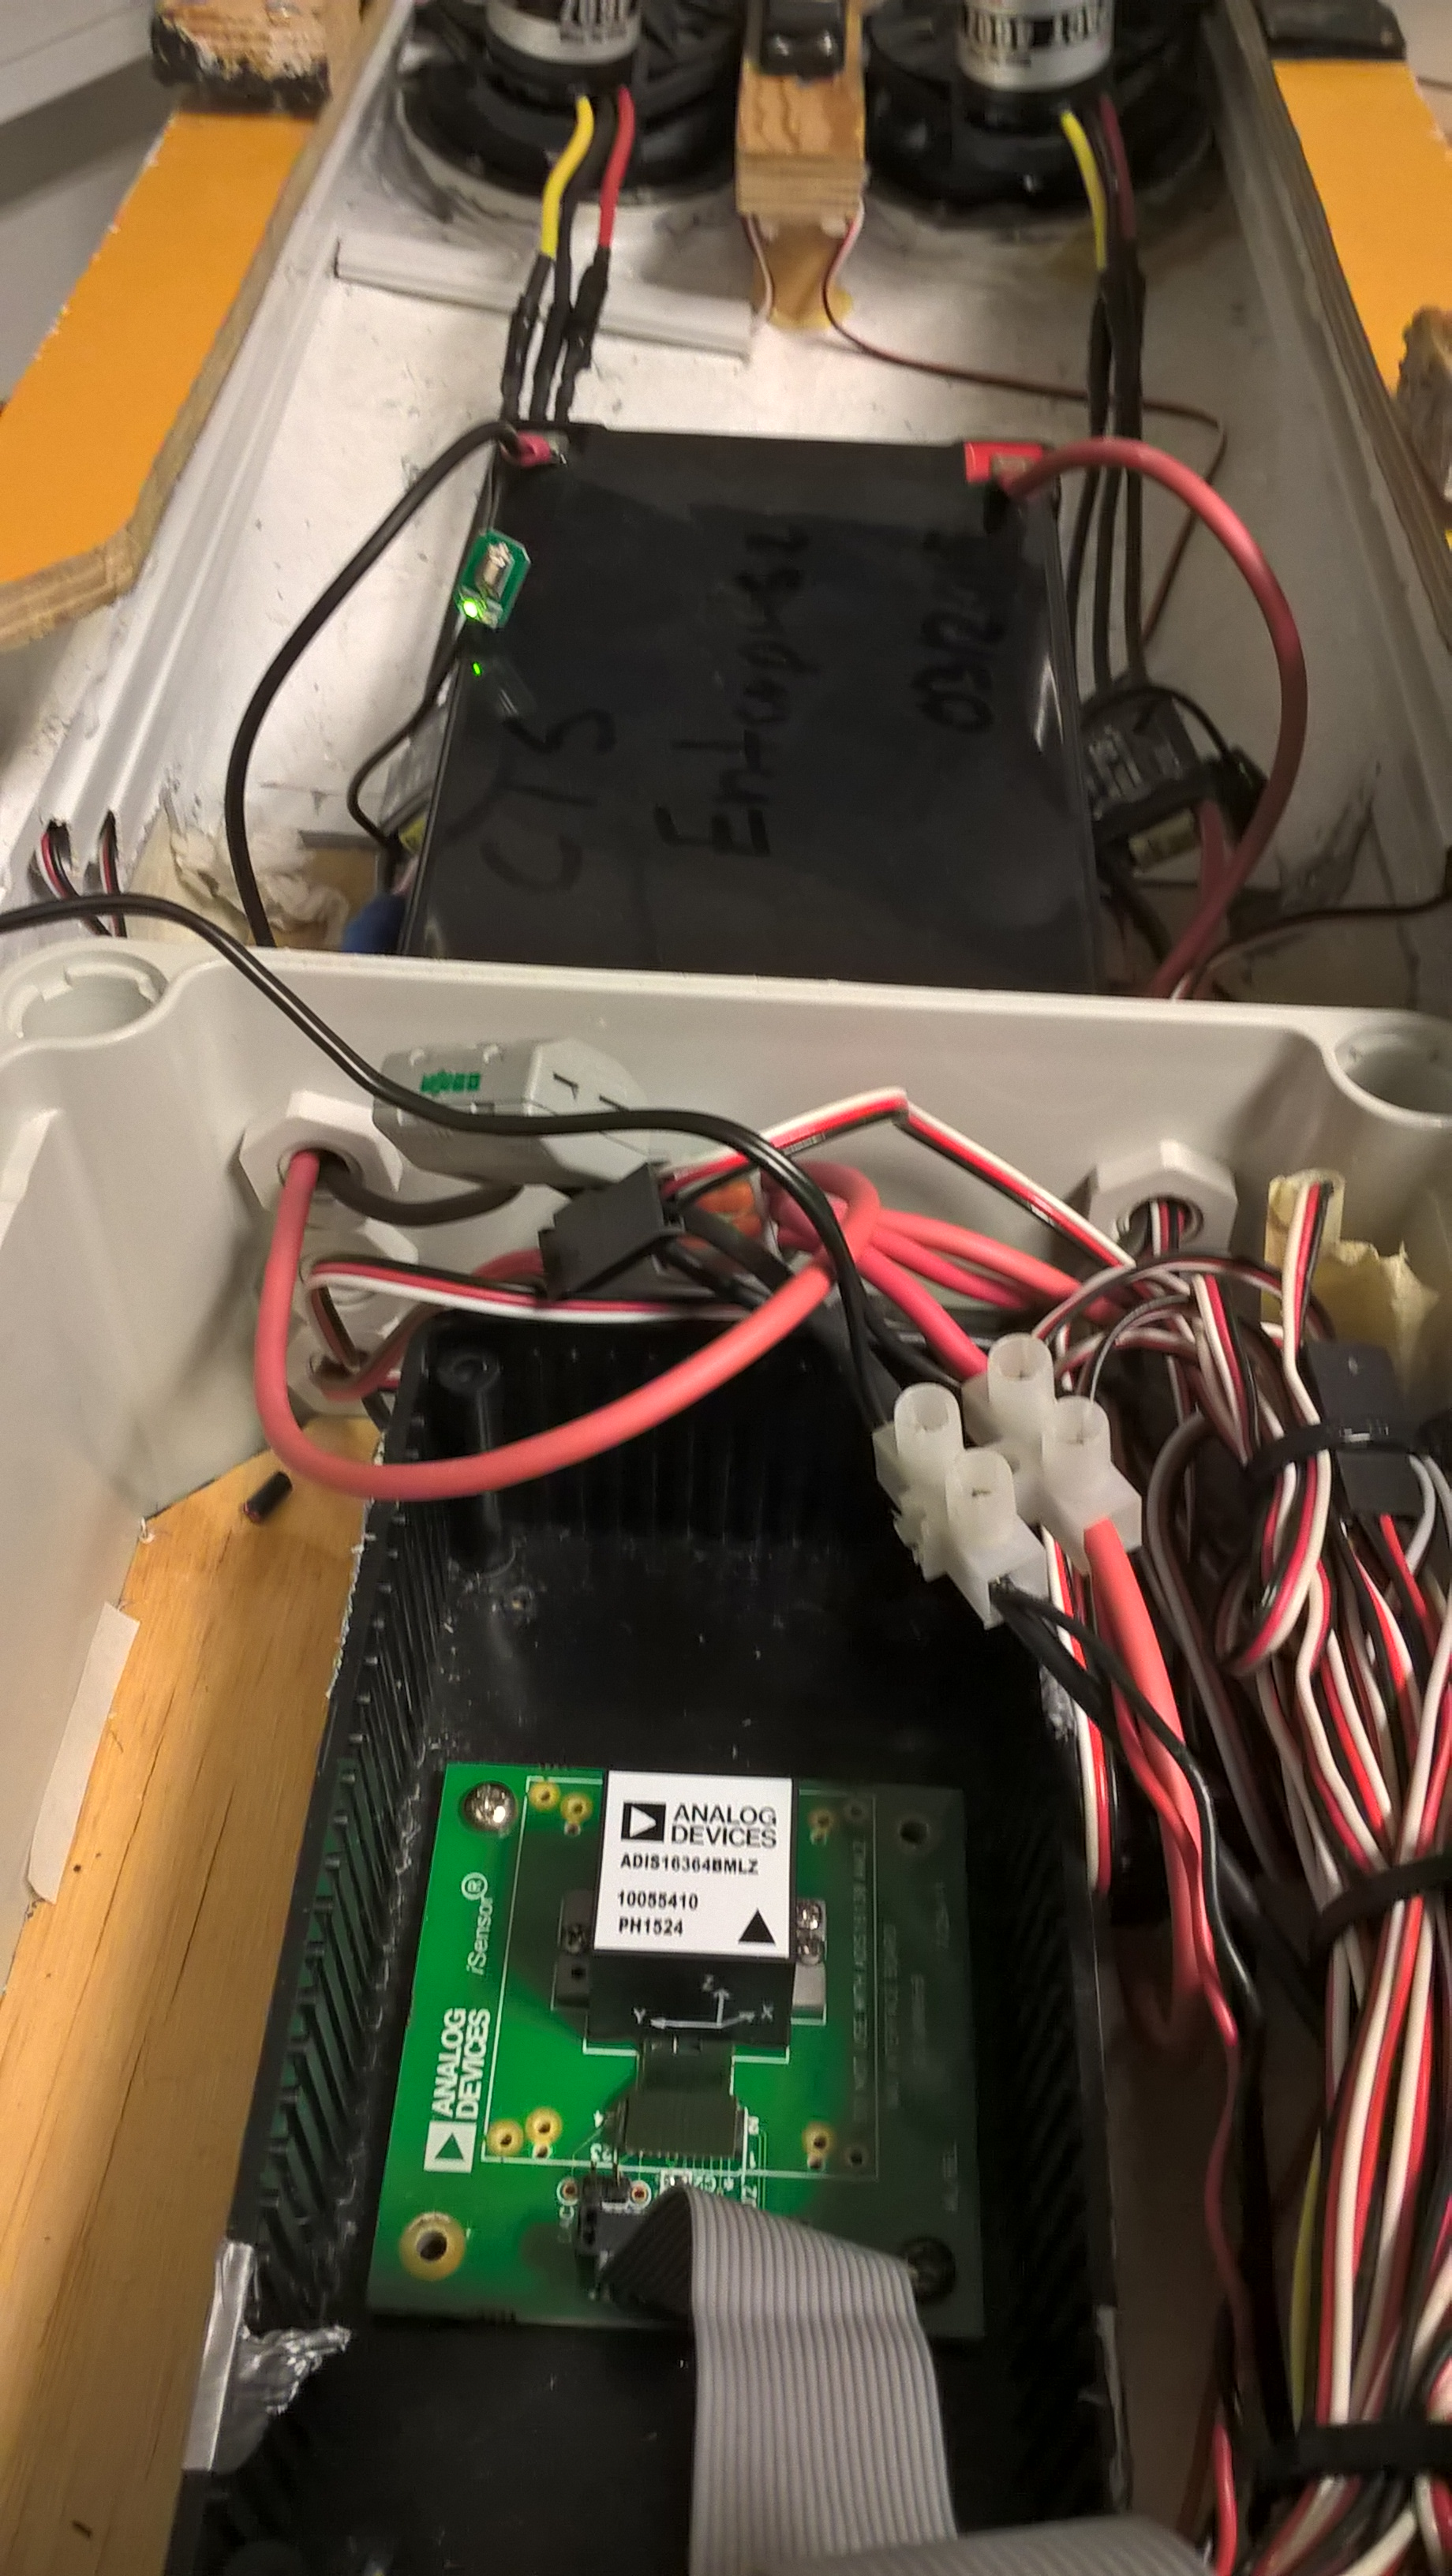
\includegraphics[width=0.9\linewidth]{fig/IMU_mounted.jpg}
		\caption{IMU mounted in the vessel}
		\label{fig:IMU_mounted}
	\end{subfigure}
\caption{Inertial Measurement Unit in CSE1}
\end{figure}

\section{Control system}
The on-board control system consists of the following parts:
\begin{itemize}
	\item a National Instruments compact reconfigurable input/output (cRIO)
	embedded controller
	\item a Raspberry Pi (RPi) single-board computer
	\item three electronic speed controllers (ESC)
	\item four servos
\end{itemize}
A short description of the cRIO and RPi is given in the latter. 
\subsection{cRIO}
The model on-board is the cRIO-9024, and it is connected to 4 FPGA modules for analogue and digital I/O:
\begin{itemize}
	\item NI-9215, used for analog input such as measuring voltage
	\item NI-9263, used for reading IMU measurements
	\item NI-9401, not used
	\item NI-9474, used for sending pwm signal
\end{itemize}
\subsection{RPi}
The Raspberry Pi provides communication with the Siaxaxis controller, as described in Section \ref{sec:high_level_communication}. It works as an embedded system, and once powered it will start searching for the wireless controller. When connection is established, it continuously sends the Sixaxis controller output to the cRIO over Ethernet. To successfully connect the sixaxis controller to the RPi, wait for the Bluetooth dongle to start blinking before pressing the PS-button on the controller. 

If there are problems establishing connection between Sixaxis and RPi, contact Torgeir Wahl or see the MCLab Handbook on Github. 

\subsection{ESC}
The ESC's are controlled with PWM signals, based on PWM tick signals. Table \ref{tab:pwm_spec} describe the setup for all ESC's on-board CSE1, and Table \ref{tab:pwm_range} gives the pwm signal range for each ESC.
\begin{table}[h!]
	\centering
	\caption{PWM specification for ESC}
	\label{tab:pwm_spec}
	\begin{tabular}{cccc}
		\hline
		\textbf{Initial value} & \textbf{Scaling} & \textbf{Offset} & \textbf{PWM period} [Ticks] \\ \hline
		0 & 100 & 0 & 800.000\\ \hline
	\end{tabular}
\end{table}

\begin{table}[h!]
	\centering
	\caption{PWM ranges for ESC}
	\label{tab:pwm_range}
	\begin{tabular}{cccc}
		\hline
		& \textbf{ESC\_BT}[\%] & \textbf{ESC\_VSP1}[\%] & \textbf{ESC\_VSP2}[\%]\\ \hline
		\textbf{min} & 7.00 & 3.12 & 3.12\\
		\textbf{neutral} & 7.55 & 5.01 & 5.01\\
		\textbf{max} & 8.10 & 6.90 & 6.90\\ \hline
	\end{tabular}
\end{table}

\section{High-level communication}\label{sec:high_level_communication}
\begin{figure}[htb!]
	\centering
	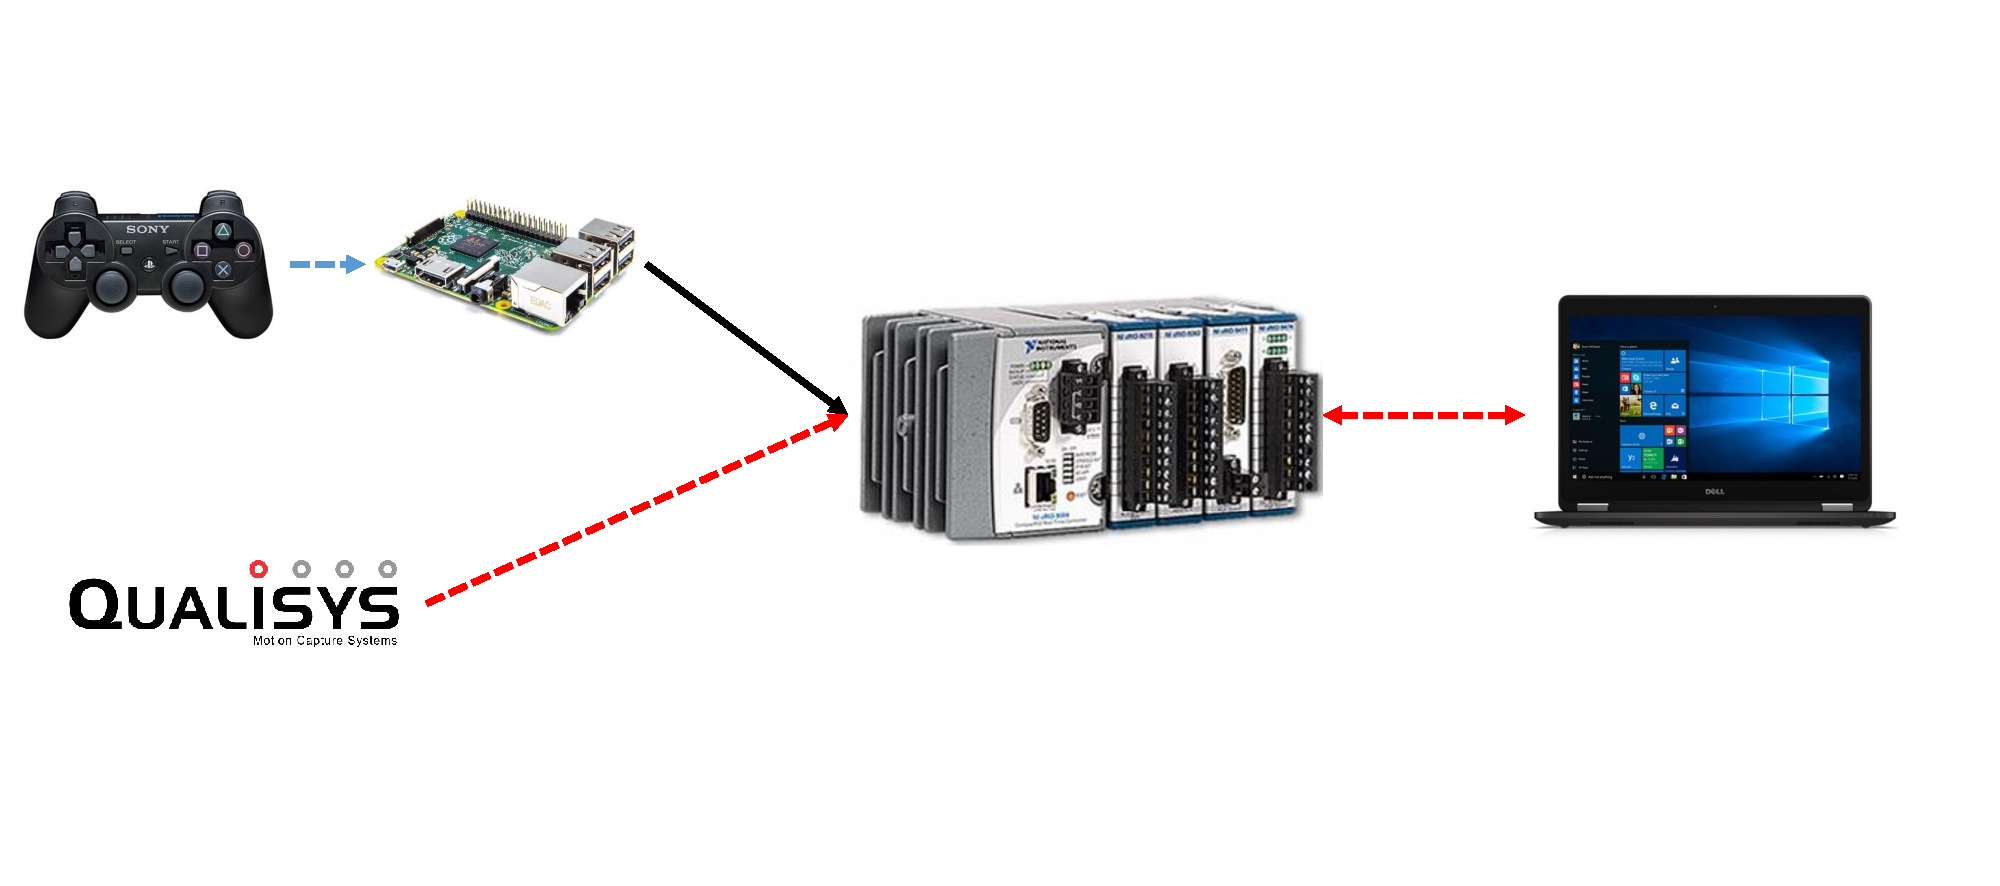
\includegraphics[width=\textwidth]{fig/high-level_control.pdf}
	\caption{CSE1 communication diagram}
	\label{fig: CSE1 communication}
\end{figure}
Following Figure \ref{fig: CSE1 communication} from left to right:
\begin{description}
	\item [{Sixaxis}] transmits its Joystick information to the RPi over Bluetooth communication. 
	\item [{RPi}] receives Sixaxis data through the USB dongle and forwards it using Ethernet connection (TCP).
	\item [{cRIO}] reads QTM broadcast positioning data through the Wi-Fi bridge on Ethernet port 1, Sixaxis data on Ethernet port 2. Online data and laptop input is transmitted and received on Ethernet port 1 by the VeriStand Engine.
	\item [{Laptop}] reads simulation data and sends input to the cRIO over MC Lab Wi-Fi.
\end{description}
Hence, there are two possible methods for controlling the vessel:
\begin{itemize}
	\item a laptop connected to the MC Lab wireless network
	\item a Sony Sixaxis wireless gamepad for PlayStation 3
\end{itemize}
Figure \ref{fig: CSE1 signal} depicts an overview of the whole communication structure of CSE1, from user input to actuator control. 
\begin{figure}[htb!]
	\centering
	\includegraphics[height=0.4\paperheight]{fig/"CSE1 signal".png}
	\caption{CSE1 signal paths}
	\label{fig: CSE1 signal}
\end{figure}

\chapter{Software}
\section{Introduction}
In order to control CSE1, there are several software parts that runs. This chapter gives a description of the software hierarchy on CSE1. Note that the software is ready to use, and alterations in the software described here is not necessary(except modifying ctrl\textunderscore custom, as described in Part \ref{part2}).
\section{Control system}
Figure \ref{fig: CSE1 software} illustrate the software architecture, and gives an overview of how the different modules are connected and the I/O from the Simulink models. In general, the software can be divided into 2 groups: 
\begin{itemize}
	\item[MATLAB] generated parts: ctrl\textunderscore custom, ctrl\textunderscore DP, ctrl\textunderscore sixaxis2thruster and u2pwm
	\item[LabVIEW] generated parts: IMU, Oqus, WL\textunderscore Joystick and FPGA
\end{itemize}
All of these modules are described in the latter. 
\begin{figure}[htb!]
	\centering
	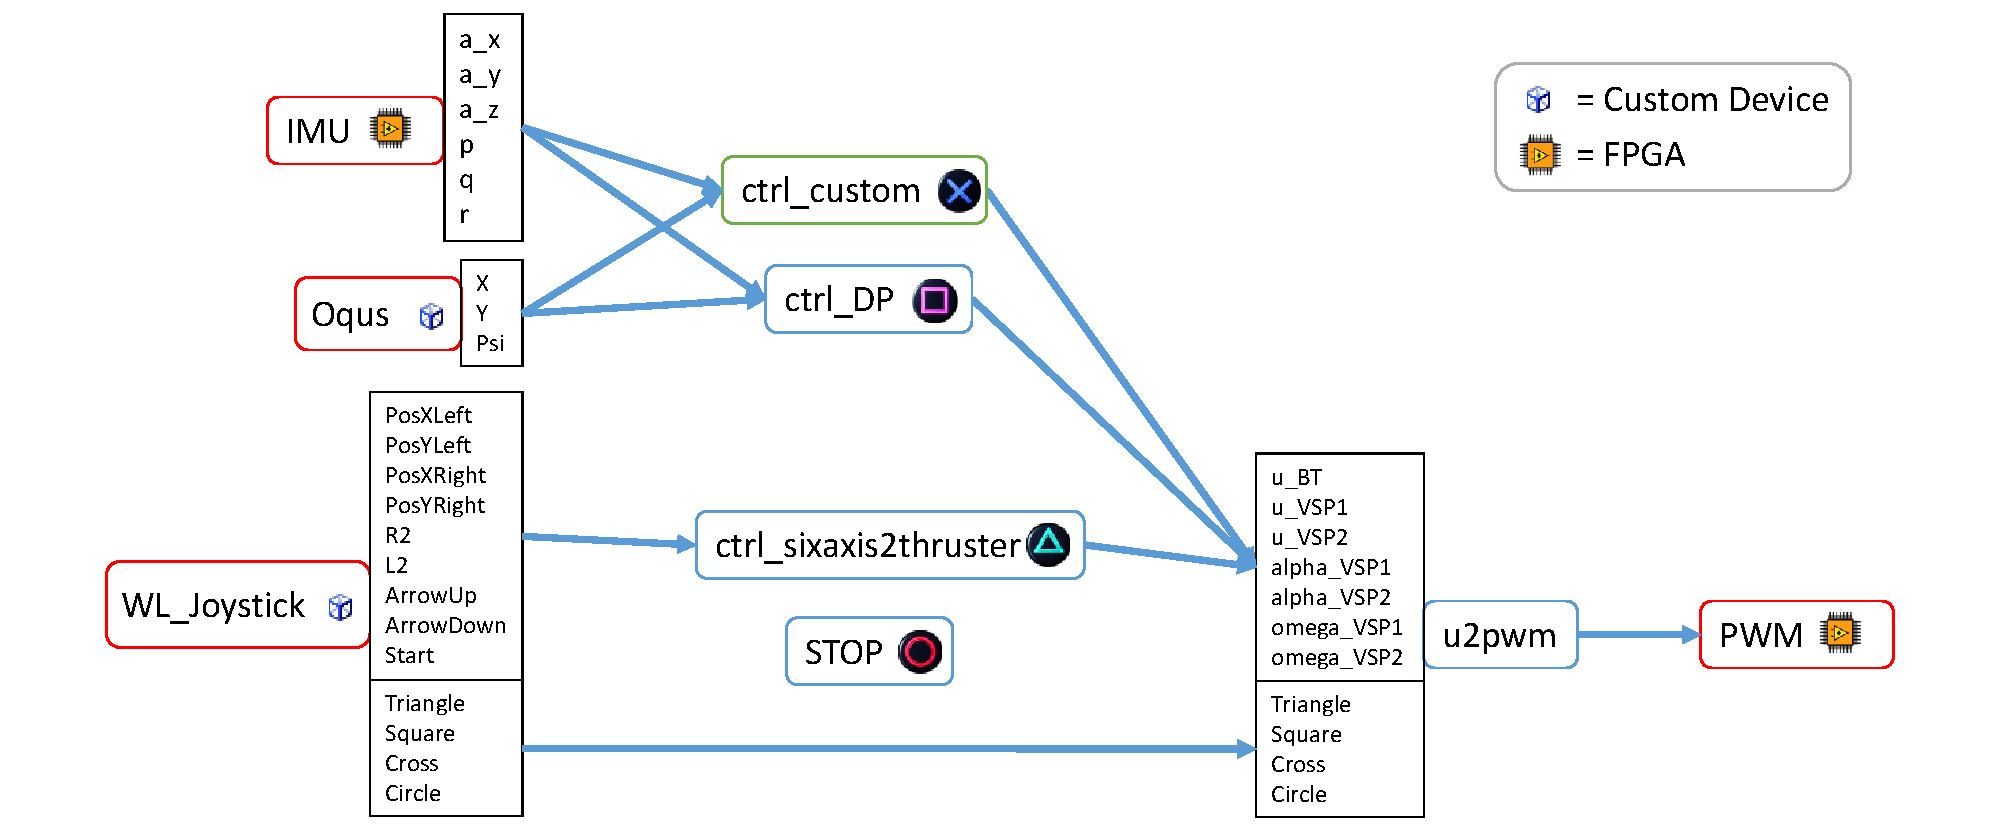
\includegraphics[width=\textwidth]{fig/software_overview.pdf}
	\caption{CSE1 control software}
	\label{fig: CSE1 software}
\end{figure}

\subsection{ctrl\textunderscore custom}
This is the only reconfigurable software, and does not consist of any control system. In Part \ref{part2} a description on how to configure and upload the code to CSE1 is given. 
\subsection{ctrl\textunderscore DP}
This code is provided as a black-box DP system, intended for demonstrations of the vessel. The desired position of the vessel is modified in VeriStand. 
\subsection{ctrl\textunderscore sixaxis2thruster}
All 3 thruster can be controlled manually using the Sixaxis controller. The right joystick control the starboard VSP, the left joystick control the port VSP and R2/L2 control the BT. The thrust limits are controlled with ArrowUp and ArrowDown, while Start is a reset button. 
\subsubsection{Voith Schneider Propellers}
\begin{figure}[!h]
	\centering 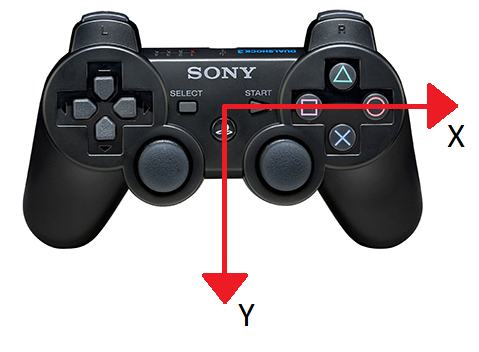
\includegraphics[width=0.5\textwidth]{fig/sixaxis_frame.png}
	\caption{Sixaxis coordinate system}
	
	\label{fig: sixaxis coordinate system} 
\end{figure}
The left and right joysticks, repectively, give the VSP deflections, $u_{\text{VSP1}}$ and $u_{\text{VSP2}}$, and angles, $\alpha_{\text{VSP1}}$ and $\alpha_{\text{VSP2}}$. The joystick coordinates PosX and PosY axes point right and down, as seen in Figure \ref{fig: sixaxis coordinate system}. The deflection is
\[
u_{\text{VSP}i}=\min\left(\sqrt{\left(\text{PosX}\right)^{2}+\left(\text{PosY}\right)^{2}},1\right).
\]
The $\min\left(\cdot\right)$ ensures constraining $u_{\text{VSP}i}\in\left[0,1\right]$. The angle is
\[
\alpha_{\text{VSP}i}=\arctan2\left(\text{PosX},-\text{PosY}\right).
\]
The VSP rotational speeds, $\omega_{\text{VSP1}}$ and $\omega_{\text{VSP2}}$, are set in $\pm0.1$ increments by use of the directional pad up and down buttons.
\subsubsection{Bow thruster}
BT is controlled by L2 and R2. Both buttons output -1 when released and increasing to 1 when fully pushed. The thruster input
\[
u_{\text{BT}}=-\frac{L2-R1}{2}
\] maps to the interval $u_{\text{BT}}\in\left[-1,1\right]$ with positive direction according towards starboard. 
\subsection{ctrl\textunderscore sixaxis2direction}
The final control mode is a basin fixed manual control of the vessel. The reference coordinate frame is defined with origin in the command center, positive x-direction towards the basin and positive y-direction towards the large towing tank. The position of the vessel is controlled with the right joystick and yaw is controlled with R2/L2. ArrowUp and ArrowDown sets the thruster limits. 
\subsection{u2pwm}
This code transforms the control input to PWM signals, which are sent to the FPGA module. There are 2 groups of inputs, namely the control signal and a switch signal. The switch signal is used to switch between the 4 control systems described in the previous. Switching is simply achieved by pressing either one of the four symbols, and the mapping between the buttons and models is shown in Figure \ref{fig: CSE1 software}. The code is not supposed to be altered, and should work as it is. The code performs four operations on the input signal, as illustrated in Figure \ref{fig:u2pwm_overview}. All four operations are explained in the latter. 
\begin{figure}[htb!]
	\centering
	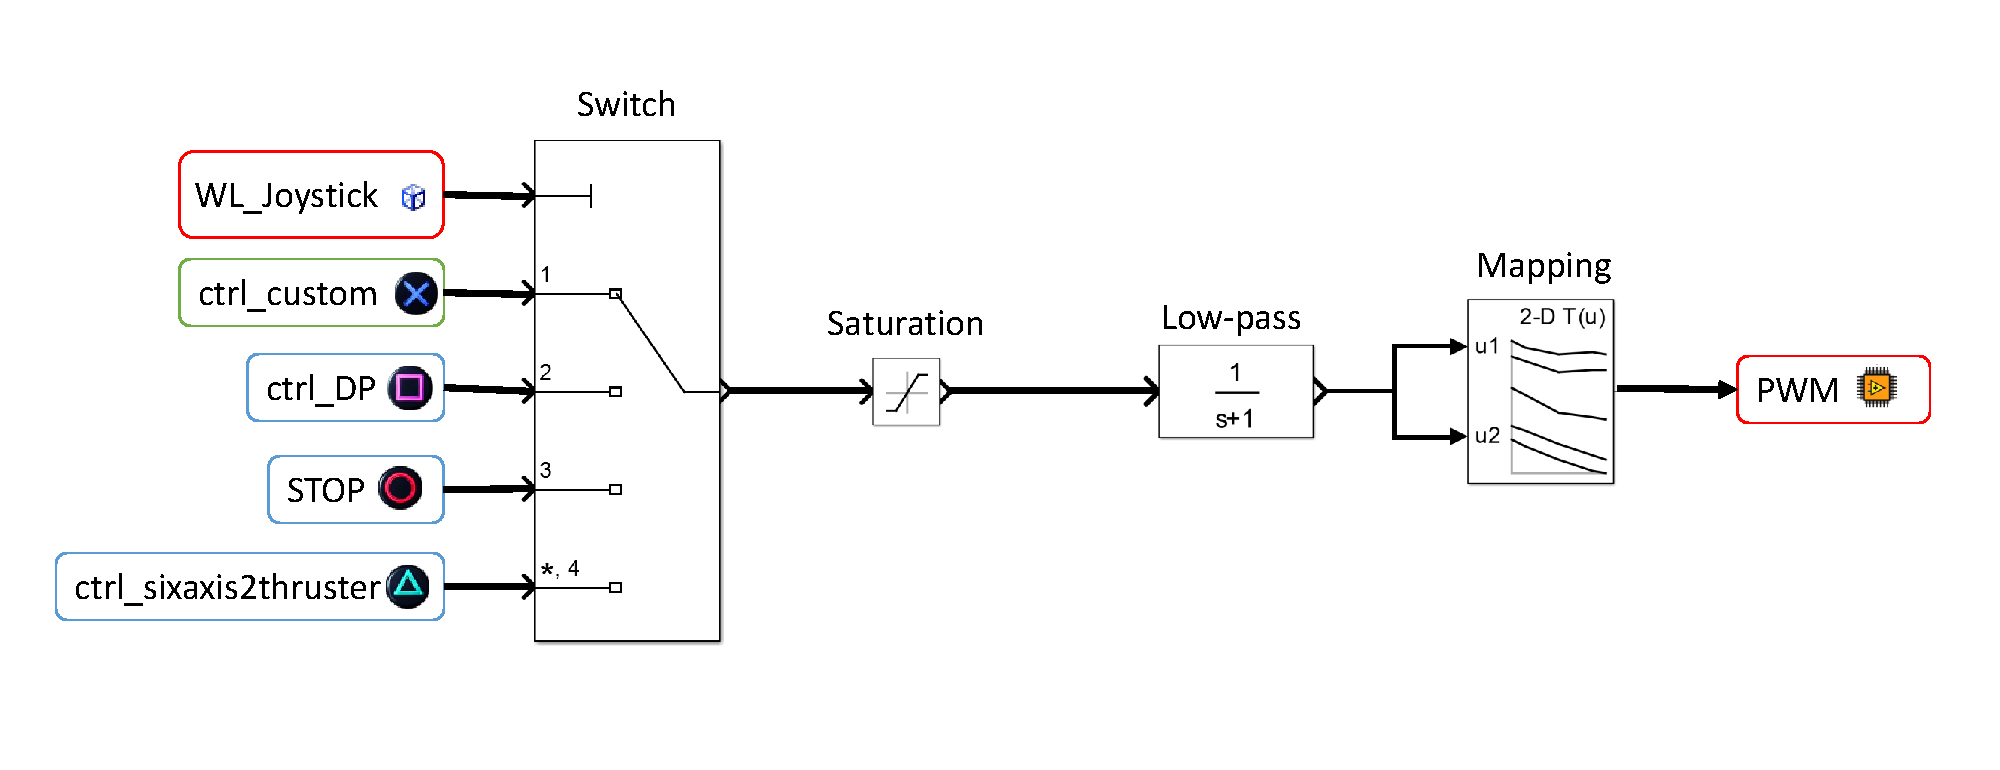
\includegraphics[width=\linewidth]{fig/u2pwm.pdf}
	\caption{Operations in u2pwm}
	\label{fig:u2pwm_overview}
\end{figure}
\subsubsection{Switch}
The switch simply forward the input from the desired model, as given by the switch signal:
\begin{itemize}
	\item ctrl\_sixaxis2thruster when 
\includegraphics[scale=0.4]{fig/sixaxis_triangle} is pushed
	\item ctrl\_DP when 
\includegraphics[scale=0.4]{fig/sixaxis_square} is pushed
	\item ctrl\_custom when 
\includegraphics[scale=0.4]{fig/sixaxis_cross} is pushed
	\item STOP when 
\includegraphics[scale=0.4]{fig/sixaxis_circle} is pushed
\end{itemize}
\subsubsection{Saturation}
The input is saturated as given in Table \ref{tab:input_saturation}. 
\begin{table}
	\caption{Control input ranges}
	\centering
	\begin{tabular}{ccc}
		\toprule 
		min & control input & max\tabularnewline
		\midrule
		$-1\leq$ & u\_BT & $\leq1$\tabularnewline
		$0\leq$ & u\_VSP1 & $\leq1$\tabularnewline
		$0\leq$ & u\_VSP2 & $\leq1$\tabularnewline
		$-\pi\leq$ & alpha\_VSP1 & $\leq\pi$\tabularnewline
		$-\pi\leq$ & alpha\_VSP2 & $\leq\pi$\tabularnewline
		$0\leq$ & omega\_VSP1 & $\leq0.4$\tabularnewline
		$0\leq$ & omega\_VSP2 & $\leq0.4$\tabularnewline
	\end{tabular}
	\label{tab:input_saturation}
\end{table}
\subsubsection{Low-pass}
The Low-pass block provides an optional simulation of a mechanical system. Modeling the system as a mechanical system is initialized in VeriStand, and must be activated by the user(default is no mechanical simulation). The time constant is equal for all parameters, and is set to 1. 
\subsubsection{Mapping}
This block converts the controller inputs to signals suitable for PWM output to the ESC. The position of the VSP steering rods are controlled by a pair of servos for each. There is a nonlinear relation between the input and the PWM signal, and thus a mapping is utilized. The constants found here are manually tuned, and if the thrusters are not operating as desired, it may be necessary with to tune the servos again. The tuning process is described below. 

\begin{table}[h!]
	\caption{Servo PWM ranges (tuned July 2017)}
	\centering
	\begin{tabular}{lllll}
		\toprule 
		\multirow{2}{*}{Position} & \multicolumn{2}{c}{VSP1} & \multicolumn{2}{c}{VSP2}\tabularnewline
		\cmidrule{2-5} 
		& servo1 {[}\%{]} & servo2 {[}\%{]} & servo3 {[}\%{]} & servo4 {[}\%{]}\tabularnewline
		\midrule
		N & 6.80 & 7.20 & 6.00 & 4.90\tabularnewline
		NE & 7.60 & 7.10 & 5.90 & 4.30\tabularnewline
		E & 7.80 & 6.50 & 5.00 & 3.80\tabularnewline
		SE & 7.60 & 5.60 & 4.30 & 4.50\tabularnewline
		S & 6.40 & 5.10 & 4.00 & 5.40\tabularnewline
		SW & 5.50 & 5.30 & 4.00 & 6.20\tabularnewline
		W & 5.20 & 5.90 & 4.60 & 6.50\tabularnewline
		NW & 5.90 & 6.80 & 5.50 & 5.80\tabularnewline
		\midrule
		Origo & 6.59 & 6.19 & 4.79 & 5.01\tabularnewline
	\end{tabular}
	\label{tab: CSE1 servo ranges} 
\end{table}

\begin{figure}[htb!]
	\centering
	
	\begin{subfigure}{.3\textwidth}
		\centering\begin{tikzpicture}
		\node[anchor=south west,inner sep=0] at (0,0) {\includegraphics[width=0.7\textwidth]{fig/"CSE1 servo settings 1".jpg}};
		\end{tikzpicture}\caption{Measurments}\label{fig: Servo measurements}\end{subfigure}
	~
	\begin{subfigure}{.3\textwidth}
		\centering\begin{tikzpicture}
		\node[anchor=south west,inner sep=0] at (0,0) {\includegraphics[width=0.7\textwidth]{fig/"CSE1 servo settings 2".jpg}};
		\end{tikzpicture}\caption{First interpolation and extrapolation}\label{fig: Servo first extrapolation}\end{subfigure}
	~
	\begin{subfigure}{.3\textwidth}
		\centering\begin{tikzpicture}
		\node[anchor=south west,inner sep=0] at (0,0) {\includegraphics[width=0.7\textwidth]{fig/"CSE1 servo settings 3".jpg}};
		\end{tikzpicture}\caption{Second extrapolation}\label{fig: Servo second extrapolation}\end{subfigure}
	
	\caption{Servo, rod position tuning}
\end{figure}

\paragraph{Tuning of servos}
One need to carry out two processes when tuning the servos, namely finding origin with the vessel floating and determining extrema with the vessel in its rack. The pwm mapping is given in Section \ref{sec:FPGA}. Finding servo extrema:
\begin{enumerate}
	\item In VeriStand, disconnect all mappings from the simulation model u2pwm to the FPGA pwm, such that thrusters and servos don't run. 
	\item In the Workspace (CSE1.nivsscreen), make 4 new numerical controls linked to the pwm signal for the servos(pwm4-pwm7). Set the scale to 100 in these controls, for higher precision when tuning. 
	\item Deploy the project, and set all 4 servos to neutral position in the numerical control. For example, if servo1 has origin in pwm=4.90, then set the value to 490 in the control. 
	\item Start seeking all 8 extrema manually, and write down the servo gains for all extrema. This is a manual process, and the direction of the rod corresponding to for example North is determined by eye. Keep in mind that the directions for each VSP are opposite. Thus, North corresponds to the rod pointing in negative y-direction for VSP1 and positive y-direction for VSP2(in body-frame). 
	\item When all extrema are found(N, NE, E,... NW) for the servos, continue to finding origin with the vessel in the basin. 
\end{enumerate}
Finding origin(neutral position) is done in the following way: 
\begin{enumerate}
	\item In the Workspace, place 2 new numerical controls and connect them to the FPGA pwm signal for VSPs(pwm1 and pwm2). Set the scale to 100. 
	\item In the u2pwm\_init.m file, find the VSP\_zero\_pwm and VSP\_u2pwm\_gain values. Find the pwm value corresponding to omega=0.3 (VSP\_zero\_pwm+0.3*VSP\_u2pwm\_gain = 5.57?)
	\item Launch CSE1 in the basin, and deploy the project. In the Workspace, set the servos to old neutral position, and then set the pwm signal (557?). 
	\item Once the VSPs are running, start tuning the servos to find the position when the vessel is at rest with running VSPs. This may take some time, but it should be possible to get a position where the vessel does not move. 
\end{enumerate}
When all 8 extrema positions and origin is found, insert the new values in \textit{u2pwm\_init.m}. The mapping function should work as it is, and Figure \ref{fig: Servo second extrapolation} illustrate the mapping. Open \textit{u2pwm.slx}, build the model with new servo mapping and update the simulation model in VeriStand. Finally, map the pwm output from u2pwm to FPGA pwm again. Deploy the project and verify the new servo setup. 
\subsection{Oqus}
The Qualisys Track Manager software broadcast the position data of the vessel over MC Lab Wifi. Reading these data is done on the cRIO through a Custom Device module named Oqus. The Oqus software simply listen to the network for data from QTM, and once it receives data it forward the position and orientation to the models as given in Figure \ref{fig: CSE1 software}. The Custom Device is programmed by Torgeir Wahl, and can be found on GitHub. 
\subsection{WL\textunderscore Joystick}
This is the second Custom Device that runs on the cRIO, which listen to the Ethernet 2 port for input from the RPi. It forwards this data to the respective models as given in Figure \ref{fig: CSE1 software}. The software is designed by Torgeir Wahl, and can be found on GitHub. 
\subsection{FPGA}\label{sec:FPGA}
For the CSE1, 3 FPGA modules are in use(1 for analog signals, 1 for digital signals and 1 for reading IMU data). The FPGA software is described in the MC Lab Software Handbook, and provides a guide on how to create an FPGA module. The modules can be found on GitHub, but are as standard. The PWM signal is mapped as described in Table \ref{tab:cRIO-actuator}.
\begin{table}[h!]
	\caption{PWM connections}
	\begin{centering}
		\begin{tabular}{ll}
			\toprule 
			\multicolumn{1}{l}{u2pwm} & FPGA\tabularnewline
			\midrule 
			$\text{\text{pwm}}_{\text{BT}}$ & pwm0\tabularnewline
			$\text{\text{pwm}}_{\text{VSP1}}$ & pwm1\tabularnewline
			$\text{\text{pwm}}_{\text{VSP2}}$ & pwm2\tabularnewline
			$\text{\text{pwm}}_{\text{servo1}}$ & pwm4\tabularnewline
			$\text{\text{pwm}}_{\text{servo2}}$ & pwm5\tabularnewline
			$\text{\text{pwm}}_{\text{servo3}}$ & pwm6\tabularnewline
			$\text{\text{pwm}}_{\text{servo4}}$ & pwm7\tabularnewline
			\bottomrule
		\end{tabular}
		\par\end{centering}
	\centering{}\label{tab:cRIO-actuator} 
\end{table}
\section{Connecting software}
All the different software parts described in the previous Section are connected together in VeriStand. On CSE1, VeriStand 2017 is used. In the system definition file \textit{CSE1.nivssdf}, all necessary mappings of variables are done. In addition, here the different Custom Devices, FPGA code and Simulink Models can be included. However, the standard setup should not be altered, as all necessary code and mappings is already taken care of. For description on how to implement the modified ctrl\textunderscore custom Simulink model, the reader is referred to Part \ref{part2}. 
\chapter{Modeling}
The mathematical model of CSE1 is given here, based on system identification done in previous Master's Theses. The model is valid for low-speed. The proposed control design model is
\begin{eqnarray}
\dot{\eta} & = & R\left(\psi\right)\nu\label{eq: CSE1 kinematics}\\
M\dot{\nu} & = & -C\left(\nu\right)\nu-D\left(\nu\right)\nu+\tau\label{eq: CSE1 kinetics}
\end{eqnarray}
where
\begin{itemize}
	\item the pose and velocity vectors are
	\[
	\eta=\left[\begin{array}{c}
	x\\
	y\\
	\psi
	\end{array}\right]\in\mathbb{R}^{3}\text{, and }\nu=\left[\begin{array}{c}
	u\\
	v\\
	r
	\end{array}\right]\in\mathbb{R}^{3},
	\]
	respectively. $\left(x,y\right)$ is the position and $\psi$ the
	yaw angle or heading in the basin frame. $\left(u,v\right)$ are the
	surge and sway velocities in the CSE1 vessel frame, and $r$ is the
	yaw rate.
	\item the thrust force and moment vector is
	\[
	\tau=\left[\begin{array}{c}
	X\\
	Y\\
	N
	\end{array}\right]\in\mathbb{R}^{3},
	\]
	where $\left(X,Y\right)$ is the surge and sway force vector, and
	$N$ is the yaw moment. The thrust forces and moments ranges are listed
	in Table \ref{tab: CSEI Thust Moment}.
	\begin{table}
		\begin{centering}
			\begin{tabular}{cc}
				& Max\tabularnewline
				\midrule 
				Surge $X$  & $1.03$ N\tabularnewline
				Sway $Y$  & $2.50$ N\tabularnewline
				Yaw $N$  & $0.98$ N\tabularnewline
				\bottomrule
			\end{tabular}
			\par\end{centering}
		\caption{\label{tab: CSEI Thust Moment}CSEI forces and moments given $\omega_{\text{VSP}}=0.3$}
	\end{table}
	\item the three degrees of freedom (3 DOF) rotation matrix is
	\[
	R\left(\psi\right)=\left[\begin{array}{ccc}
	\cos\psi & -\sin\psi & 0\\
	\sin\psi & \cos\psi & 0\\
	0 & 0 & 1
	\end{array}\right].
	\]
	\item the vessel inertia matrix is
	\[
	M=\left[\begin{array}{ccc}
	m-X_{\dot{u}} & 0 & 0\\
	0 & m-Y_{\dot{v}} & mx_{g}-Y_{\dot{r}}\\
	0 & mx_{g}-Y_{\dot{r}} & I_{z}-N_{\dot{r}}
	\end{array}\right]=M^{\top}>0.
	\]
	
	\item the coriolis and centripetal matrix is
	\begin{equation*}
	\textbf{C}(\bm{\nu})=\left[ \begin{tabular}{ccc}
	0 & $ 0 $ & $(-mx_g+Y_{\dot{r}})r+(-m+Y_{\dot{v}})v$\\
	0 & 0 & $(m-X_{\dot{u}})u$\\
	$(mx_g-Y_{\dot{r}})r+(m-Y_{\dot{v}})v $ & $(-m+X_{\dot{u}})u$ & 0\\
	\end{tabular} \right]
	\end{equation*}
	\item the damping matrix is
	\[
	D\left(\nu\right)=\left[\begin{array}{ccc}
	d_{11}\left(u\right) & 0 & 0\\
	0 & d_{22}\left(v,r\right) & d_{23}\left(v,r\right)\\
	0 & d_{32}\left(v,r\right) & d_{33}\left(v,r\right)
	\end{array}\right],
	\]
	where the damping components are 
	\begin{eqnarray}
	d_{11}\left(u\right) & = & -X_{u}-X_{\left\vert u\right\vert u}\left\vert u\right\vert -X_{uuu}u^{2}\label{Eq:d11}\\
	d_{22}\left(v,r\right) & = & -Y_{v}-Y_{\left\vert v\right\vert v}\left\vert v\right\vert -Y_{vvv}v^{2}-Y_{\left\vert r\right\vert v}\left\vert r\right\vert \label{Eq:d22}\\
	d_{23}\left(v,r\right) & = & -Y_{r}-Y_{\left\vert v\right\vert r}\left\vert v\right\vert -Y_{\left\vert r\right\vert r}\left\vert r\right\vert -Y_{rrr}r^{2}\label{Eq:d23}\\
	d_{32}\left(v,r\right) & = & -N_{v}-N_{\left\vert v\right\vert v}\left\vert v\right\vert -N_{vvv}v^{2}-N_{\left\vert r\right\vert v}\left\vert r\right\vert \label{Eq:d32}\\
	d_{33}\left(v,r\right) & = & -N_{r}-N_{\left\vert v\right\vert r}\left\vert v\right\vert -N_{\left\vert r\right\vert r}\left\vert r\right\vert -N_{rrr}r^{2}\label{Eq:d33}
	\end{eqnarray}
\end{itemize}
The rigid body inertia and hydrodynamic added mass parameters are given in Table \ref{tab: CSE1-rigid-body}, and the hydrodynamic damping parameters are given in Table \ref{tab: CSE1 damping parameters 2}.
\begin{table}[h!]
	\begin{centering}
		\begin{tabular}{crcr}
			\multicolumn{2}{c}{Rigid body} & \multicolumn{2}{c}{Added mass}\tabularnewline
			\midrule 
			Parameter & Value & Parameter & Value\tabularnewline
			\midrule 
			$m$  & $14.11$  & $X_{\dot{u}}$  & $-2$ \tabularnewline
			$I_{z}$  & $1.76$  & $Y_{\dot{v}}$  & $-10$ \tabularnewline
			$x_{g}$  & $0.0375$  & $Y_{\dot{r}}$  & $-0$ \tabularnewline
			$y_{g}$  & $0.0$  & $N_{\dot{r}}$  & $-1$ \tabularnewline
			\bottomrule
		\end{tabular}
		\par\end{centering}
	\caption{CSE1 rigid body and added mass parameters}
	\label{tab: CSE1-rigid-body}
\end{table}

\begin{table}[h!]
	\begin{centering}
		\begin{tabular}{crcrcr}
			\multicolumn{2}{c}{Hydro surge} & \multicolumn{2}{c}{Hydro sway} & \multicolumn{2}{c}{Hydro yaw}\tabularnewline
			\midrule 
			{Parameter}  & {Value}  & {Parameter}  & {Value}  & {Parameter}  & {Value} \tabularnewline
			\midrule 
			$X_{u}$  & $-0.6555$  & $Y_{v}$  & $-1.33$  & $N_{v}$  & $0.0$ \tabularnewline
			$X_{uu}$  & $0.3545$  & $Y_{vv}$  & $-2.776$  & $N_{vv}$  & $-0.2088$ \tabularnewline
			$X_{uuu}$  & $-3.787$  & $Y_{vvv}$  & $-64.91$  & $N_{vvv}$  & $0.0$ \tabularnewline
			$X_{v}$  & $0.0$  & $Y_{r}$  & $-7.25$  & $N_{r}$  & $-1.9$ \tabularnewline
			$X_{vv}$  & $-2.443$  & $Y_{rr}$  & $-3.45$  & $N_{rr}$  & $-0.75$ \tabularnewline
			$X_{vvv}$  & $0.0$  & $Y_{rrr}$  & $0.0$  & $N_{rrr}$  & $0.0$ \tabularnewline
			$.$  & $.$  & $Y_{rv}$  & $-0.805$  & $N_{rv}$  & $0.130$ \tabularnewline
			$.$  & $.$  & $Y_{vr}$  & $-0.845$  & $N_{vr}$  & $0.080$ \tabularnewline
			\bottomrule
		\end{tabular}
		\par\end{centering}
	\caption{CSE1 damping parameters}
	\label{tab: CSE1 damping parameters 2}
\end{table}